\chapter{The MAC layer}

\section{Introduction}

The MAC layer handles access to the same medium, avoiding collisions that cause
waste of time.
It has the following goals:
\begin{itemize}
\item Efficency in bandwith use
\item Avoid collisions (resilience)
\item Fairness
\item Robustness: the protocol should be decentralized
\item Protocols easy to implement
\end{itemize}

\paragraph*{Typologies} The MAC layer has different typologies. As a matter of
fact, it offers different
ways to share the channel: \textbf{TDMA} (\textit{time division}), \textbf{FDMA}
(\textit{frequency division}), \textbf{CDMA} (\textit{time division}).
\paragraph*{Random access} MAC provides two way to randomly access the channel,
with \textbf{CSMA}
(\textit{carrier sense multiple access} and MACA (\textit{multiple access with
  collision avoidance}).
\paragraph*{Other protocols} There are also ``taking turns'' MAC protocols, that
basically carries out a
polling scheme.

\subsection{Wired vs Shared Channel}

When the channel is a cable it's easier, because you just have to listent to it
before trasmitting an data (this techinque is called CSMA, \textit{Carrier sense
  multiple access}\footnote{As an additional note, with CSMA you can even listen
  when a collision happens.}). In a wireless environment this is not possible,
because when you're transmitting you can't receive, otherwise you'll end up
having a collision.

\section{MAC Layer approaches}

There are different ways the MAC layer can approach the access to the medium,
and these are:
\begin{itemize}
\item Random
  \begin{itemize}
  \item without carrier sensing (such as Aloha, Slotted Aloha)
  \item with carrier sensing (CSMA, CSMA/CD, MACAW)
  \end{itemize}
\item Controlled
  \begin{itemize}
  \item centralized (FDMA, TDMA, CDMA)
  \item distributed
  \end{itemize}
\end{itemize}

\subsection{Aloha}

This protocols was used to communicate between Hawaii islands. It doesn't have
synchronization, and the total thoughput of this protocols is $\frac{1}{2}e$

\subsubsection{Slotted Aloha}

This version of Aloha has time divided slots: every transmission has to stay in
a defined time slot, that is not easy to do but it's possible. In case of a
collision, a retransmission occurs with a probability $P$.

\paragraph*{Thoughput} The thoughput of this Aloha version with synchronization
is $\frac{1}{e}$

\subsubsection{Considerations about Aloha protocols}

In general, Aloha protocols have these common characteristics:
\begin{itemize}
\item not efficent
\item unfair
\item robust \& easy to implement
\end{itemize}

\subsection{CSMA}

With this approach, you first listen to the channel and then the protocol
algorithm tries to avois transmission at the same time. CSMA comes with
different versions, based on the probability $p$ of trasmission after the
channel becomes free.

\paragraph*{1-persistent CSMA} When the channel is free $\to$ transmit,
otherwise, wait until the channel becomes free. At this point, immediatly
transmit. If a collision occurs, wait a random amount of time before
retransmission.

It's easy to see that if two nodes are waiting the channel to become free they
will probably cause a collision because they will start transmitting at the
same time.

\paragraph*{non-persistent CSMA} Similar to 1-persistent CSMA, but if the
channel is busy then wait a random amount of time before checking it again.

\paragraph*{p-persistent CSMA} This version is slot based. If the channel is
free then the node transmits with a probability $p$, otherwise it waits a random
amount of time.

\subsubsection{CSMA/CD}

The CD version has a collision detection system, that allows to abort the
transmission when a collision is detected, reducing time wastage. This,
unfortunatly, is \underline{not possible in wireless communications}, but only
in the wired one.

\paragraph*{SINR} The collision detection is based on the SINR
(\textit{signal-to-interference-plus-noise ratio}). The formula to calculate
SINR is:
\begin{equation}
SINR = \frac{Signal\ of\ Interest\ (SoI)}{Interference(I) + Noise(N)}
\end{equation}

The formula to calculate the SINR between two nodes (given intereference between
C and B) is:
\begin{equation}
SINR^{A}_{B} = \frac{\frac{P^{A}_{transmit}}{d^{\alpha}_{AB}}}{N + \frac{P^{C}_{transmit}}{d^{\alpha}_{CB}}}
\end{equation}

\begin{figure}[t]
  \centering
  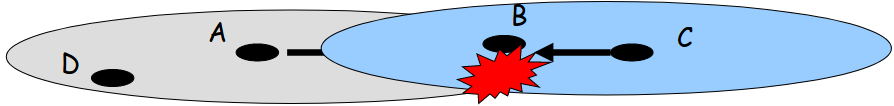
\includegraphics[scale=0.4]{SINR1}
  \caption{An example of a collision detection}
\end{figure}

In this formula $P^{X}_{transmit}$ represents the power transmission of X, and
$d^{\alpha}_{XY}$ is the \textit{SoI} between $X$ and $Y$. The noise ($N$) is
somehow a fixed value.

The nodes position and the signal interferences cause communication problems in
wireless networks, e.g. the \textbf{Hidden terminal problem} and the \textbf{
  exposed terminal problem}, that will be explained in the next part.

\section{Communication problems with wireless networks}

As already mentioned, there are problems with wireless networks related to the nodes' position and the strenght of the signal that will be explained here.

\subsection{Hidden terminal problem}

The hidden node problem occurs when a node is visible from a wireless access
point (AP) but not from other nodes communicating with that AP, due to
difficulties in the media access control sublayer.

\begin{figure}[t]
  \centering
  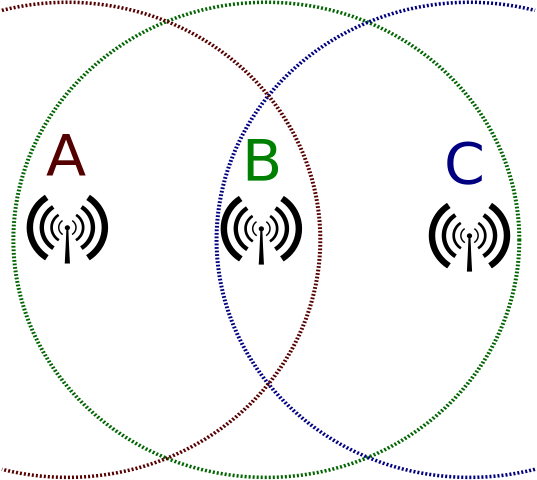
\includegraphics[scale=0.25]{WifiHiddenStationProblem}
  \caption{Hidden terminal problem. Station A can communicate with Station B.
    Station C can also communicate with Station B. However, Stations A and C
    cannot communicate with each other since they cannot sense each other on
    the network, because they are out of range of each other.}
\end{figure}

\subsection{Exposed terminal problem}

Exposed node problem occurs when a node is prevented from sending packets to
other nodes because of a neightboring transmitter.

\begin{figure}[t]
  \centering
  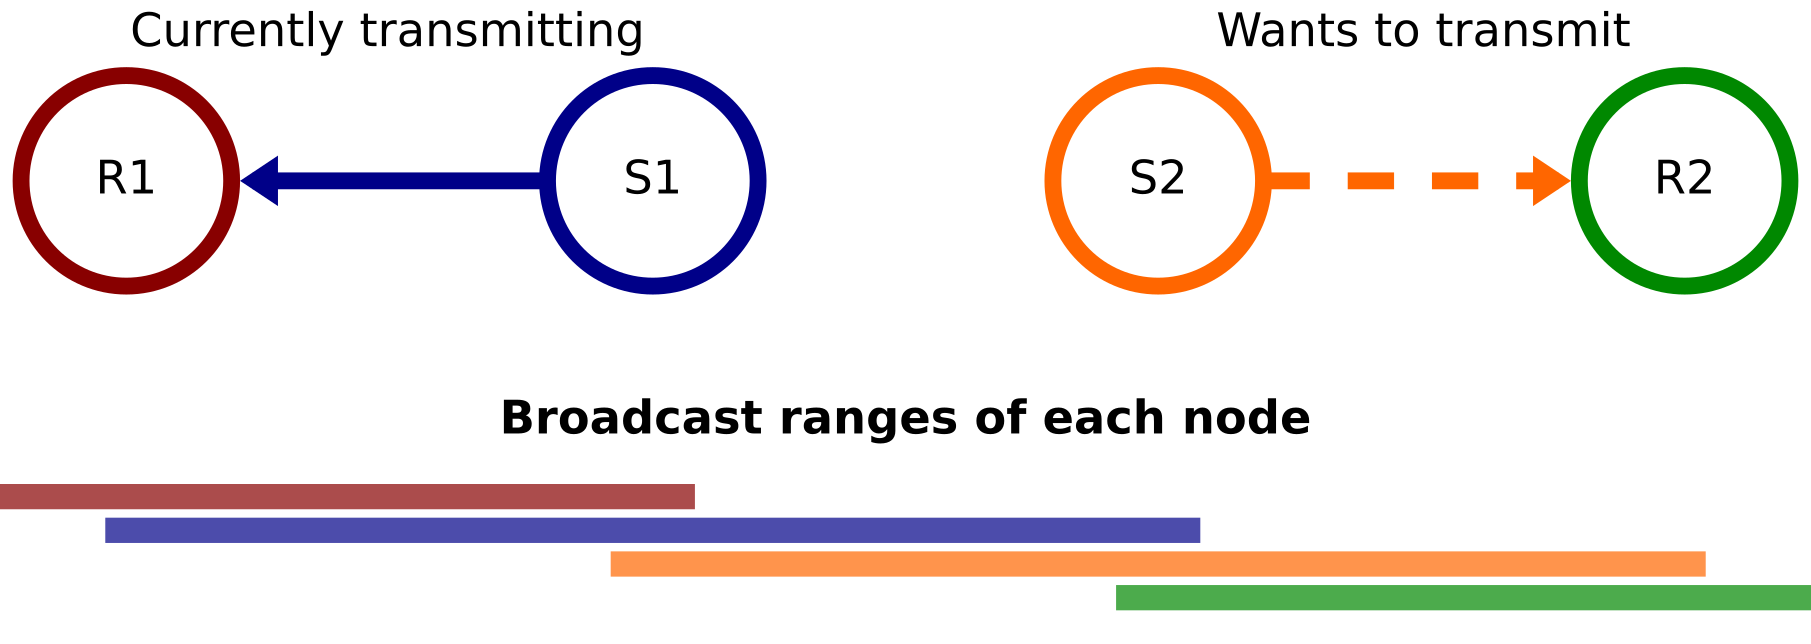
\includegraphics[scale=0.8]{WifiExposedStationProblem}
  \caption{Exposed terminal problem. Station S2 wants to communicate with R2,
    but has sensed S1 that's currently transmitting to R1 so it doesn't
    trasmit for not causing a collision. In this case, though, S2 should not
    defer trasmission to R2 because this won't create any interference with
    S1's trasmission.}
\end{figure}

\subsection{MACAW} \todo{This part is very confused, since the slides are a
  clusterfuck of infomation throwed randomly. Please check out \underline{very
    closely} and critically this content because I'm not sure of what I'm
  writing!}

Given that wireless MAC proved to be non-trivial, in 1994 a research lead by
Bhargavan made MACAW (\textit{Multiple Access with Collision Avoidance for
  Wireless}) that now is used for congestion avoidance. It has the same
operating principle of 802.11, and it's widely used in ad hoc networks.
MACAW helps solving the hidden terminal problem.

\paragraph*{How it works} WIP
